\documentclass[letterpaper, 12pt]{article}

\usepackage{graphicx}
\usepackage{longtable}
\usepackage{rotating}
\usepackage{dcolumn}
\usepackage{listings}
\usepackage{subfiles}
\usepackage{amsmath}

% Code listing commands
\lstset{language=R,
basicstyle=\scriptsize\ttfamily,
commentstyle=\ttfamily,
numbers=left,
numberstyle=\footnotesize,
stepnumber=1,
numbersep=5pt,
showspaces=false,
showstringspaces=false,
showtabs=false,
frame=single,
tabsize=2,
captionpos=b,
breaklines=true,
breakatwhitespace=false,
title=\lstname,
escapeinside={},
keywordstyle={},
morekeywords={}
}

\begin{document}
\title{ARE213 Problem Set \#2A}
\author{Peter Alstone \& Frank Proulx}
\maketitle

\section{Problem \#1}
\subsection{Part A}
Here we will consider the within estimator, as suggested. This suggests that we want to find $\widehat{\beta_{FE}}$ by running the following regression:
\begin{equation}
\ddot{Y_{it}} = \ddot{X'_{it}}\widehat{\beta_{FE}} + \ddot{\epsilon_{it}}
\end{equation}
Where $\ddot{Y_{it}}=Y_{it}-\bar{Y_i}$, $\ddot{X_{it}}=X_{it}-\bar{X_i}$, $\bar{Y_i}=\frac{1}{T}\sum_{t=1}^TY_{it}$, and $\bar{X_i}=\frac{1}{T}\sum_{t=1}^TX_{it}$.
Our fixed effects estimator is therefore

\begin{equation}
\widehat{\beta_{FE}}=(\ddot{X'_{it}}\ddot{X_{it}})^{-1}\ddot{X'_{it}}\ddot{Y_{it}} %His notes say you ``don't have to invert the mega-matrix'', so I might be doing this wrong.
\end{equation}

Because we have T=2, this can be rewritten as
\begin{equation}
\widehat{\beta_{FE}}=((X_{it}-\frac{1}{2}X_{i1}-\frac{1}{2}X_{i2})'(X_{it}-\frac{1}{2}X_{i1}-\frac{1}{2}X_{i2}))^{-1}(X_{it}-\frac{1}{2}X_{i1}-\frac{1}{2}X_{i2})'(Y_{it}-\frac{1}{2}Y_{i1}-\frac{1}{2}Y_{i2})
\end{equation}




And looking at the first differences estimator, where we get $\widehat{\beta_{FD}}$ by running the regression
\begin{equation}
\Delta Y_{it} = \Delta X'_{it} \widehat{\beta_{FD}} + \Delta \epsilon_{it}
\end{equation}

where $\Delta Y_{it} = Y_{it} - Y_{it-1}$, $\Delta X_{it} = X_{it} - X_{it-1}$, and $\Delta \epsilon_{it} = \epsilon_{it} - \epsilon_{it-1}$.

Because we only have T=2, this differencing estimator can only be estimated for t=2, so we regress
\begin{align}
\Delta Y_{i2} = \Delta X'_{i2} \widehat{\beta_{FD}} + \Delta \epsilon_{i2} \\
Y_{i2}-Y_{i1} = (X_{i2}-X_{i1})'\widehat{\beta_{FD}} + \epsilon_{i2}-\epsilon_{i1}
\end{align}

thus, our first difference estimator is
\begin{equation}
\widehat{\beta_{FD}}=((X_{i2}-X_{i1})'(X_{i2}-X_{i1}))^{-1} (X_{i2}-X_{i1})'(Y_{i2}-Y_{i1})
\end{equation}

\section{Problem \#3}
\subsection{Part A}
Running pooled bivariate OLS, adding a quadratic time trend, and adding the covariates that we expect to belong produces the models shown in Table ref{tab:3a}.  The pooled OLS is an ill-informed baseline model but nonetheless tells us that there is a statistically significant negative correlation between the states with primary seatbelt laws and those without.  In particular, the mean of the log fatalities per capita is reduced by 0.14 for states with primary seatbelt laws.  This does not, however, account for the year to year trends that are captured by including a set of quadratic year terms in the regression as shown in the ``quadratic time" regression.  This basic trend is that deaths have gone down over time.  Correcting for these trends may allow our OLS estimates approach the true ATE, and indeed the apparent effect of primary seatbelt laws is reduced.  When further covariates are added that are relevant (see Table ref{tab:3a}) further reductions in the apparent effect occur and the effect is no longer statistically significant.  
\subfile{p3a.tex}

\begin{figure}[htbp]
\begin{center}
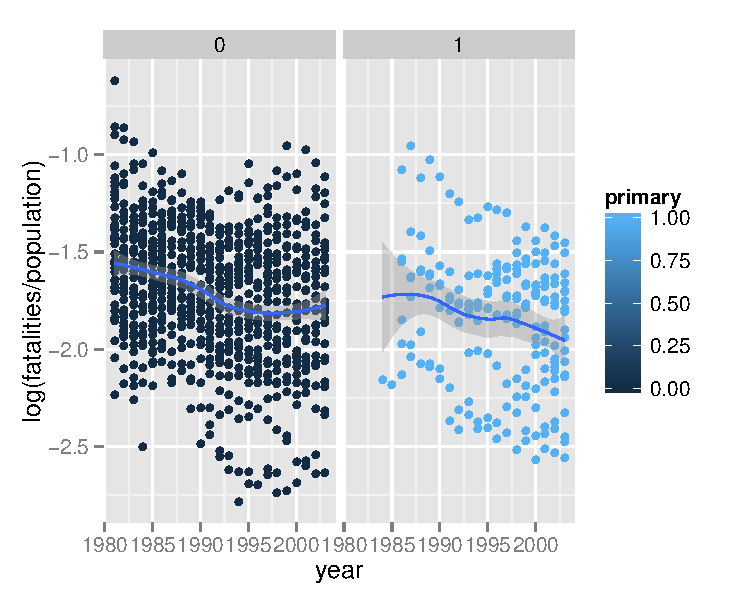
\includegraphics{plot3a.pdf}
\caption{Year to year trends in the log of traffic fatalities per capita, divided by primary seatbelt law presence.  A LOESS fit to each dataset is included for reference but is not necessarily indicative of the true underlying function.}
\label{fig:3a}
\end{center}
\end{figure}



\subsection{Part B}
No, the standard errors are most likely not correct (are they ever really correct?).  In this case the error comes from


\subsection{Part C}
The between estimator will give an unbiased estimate of the effect of primary seat belt laws insofar as variation within states (across time) is uncorrelated with the observables.
\subfile{p3c.tex}

We don't think that this criterion is met here. For example, within a given state, the total vmt per year probably tracks very closely with fatalities, as the higher VMT within a given year, the more likely there are to be fatal crashes (ceteris paribus).
%% I don't know what to say about standard errors.


\subsection{Part D}
The RE estimator will give an unbiased estimate so long as the within states variation is uncorrelated with observables. Again, this assumption is probably not met here.
\subfile{p3d.tex}

The Random Effects estimator has the advantage over pooled OLS that it allows for (and assumes) unobserved heterogeneity. OLS has the advantage that it is more efficient than the Random Effects estimator when said heterogeneity does not exist.

\subsection{Part E}

\subsection{Part F}
\subfile{p3fg.tex}


\subsection{Part G}

\end{document}
